\subsection{Selected Exercises and Tools}\label{sec:selected_exercises}

\begin{figure*}[t!]
\centering
\begin{subfigure}[t]{0.3\textwidth}
  \centering
  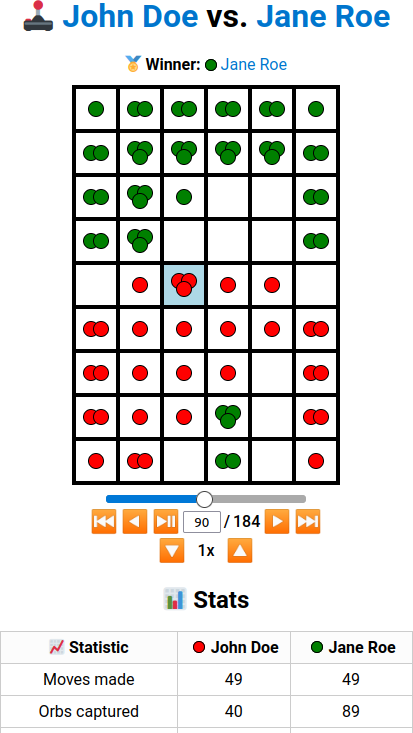
\includegraphics[width=\linewidth]{img/chainreaction}
  \caption{Game strategies and tournaments}
\end{subfigure}%
~
\begin{subfigure}[t]{0.3\textwidth}
  \centering
  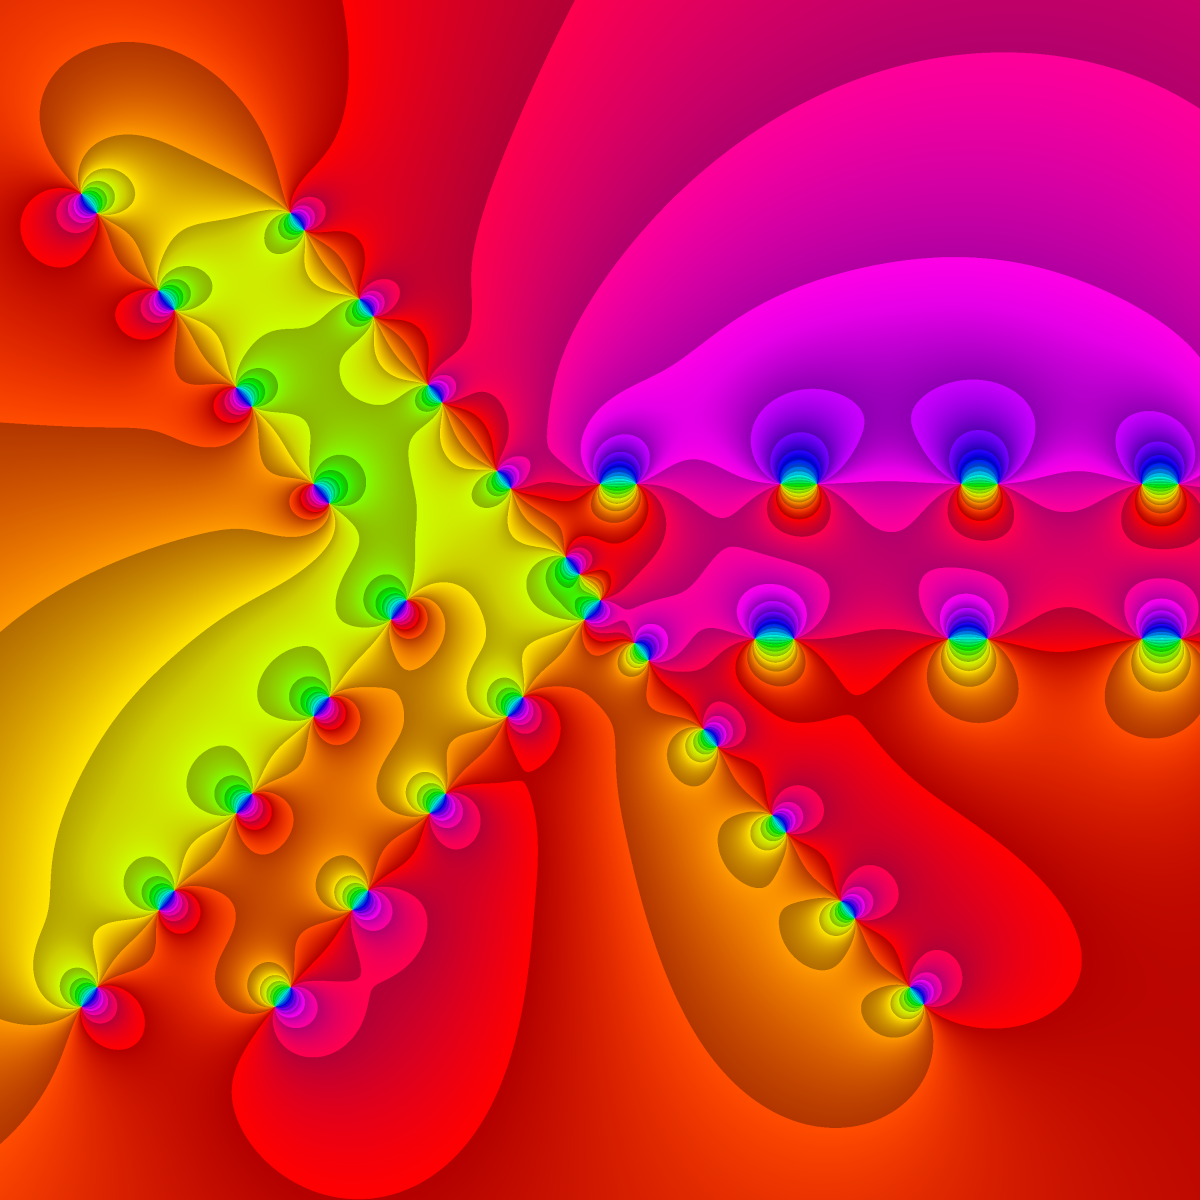
\includegraphics[width=\linewidth]{img/haskell_art}
  \caption{Art generation}
\end{subfigure}
~
\begin{subfigure}[t]{0.33\textwidth}
  \centering
  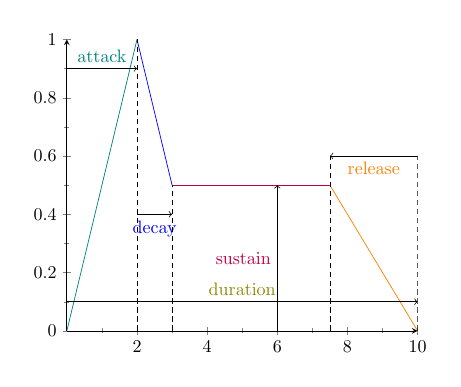
\begin{tikzpicture}[scale=0.65]
  \begin{axis}[
    minor tick num=1,
    samples=120,
    axis y line=left,
    axis x line=middle
    ]
    \addplot+[domain=0:10, mark=none, teal]
      coordinates {(0,0) (2, 1)};
    \addplot+[domain=0:10, mark=none, blue]
      coordinates {(2,1) (3, 0.5)};
    \addplot+[domain=0:10, mark=none, purple]
      coordinates {(3, 0.5) (7.5, 0.5)};
    \addplot+[domain=0:10, mark=none, orange]
      coordinates {(7.5, 0.5) (10, 0)};
    \addplot[densely dashed] coordinates {(2,0) (2,1)};
    \addplot[densely dashed] coordinates {(3,0) (3,0.5)};
    \addplot[densely dashed] coordinates {(7.5,0) (7.5,0.6)};
    \addplot[densely dashed] coordinates {(10,0) (10,0.6)};
    \addplot[->] coordinates {(0,0.9) (2,0.9)} node[midway, above, teal] {attack};
    \addplot[->] coordinates {(2,0.4) (3,0.4)} node[midway, below, blue] {decay};
    \addplot[->] coordinates {(6,0) (6,0.5)} node[midway,left, purple] {sustain};
    \addplot[<-] coordinates {(7.5,0.6) (10,0.6)} node[midway, below, orange] {release};
    \addplot[->] coordinates {(0,0.1) (10,0.1)} node[midway, above, olive] {duration};
  \end{axis}
  \end{tikzpicture}
  \caption{Music synthesis}
\end{subfigure}
\caption{Examples of exercises created as part of the course}
\end{figure*}

Many students at TUM have questioned the
applicability and usefulness
of functional languages after completing
their mandatory functional programming course.
We believe this is mainly due to two reasons:
1) introductory programming courses often stick
to simple algorithmic or mathematically inspired challenges and
2) side-effects (in particular IO)
are often introduced very late
in functional programming courses.

Changing the latter appeared unpromising to us:
we think that students would be confused
if a ``special'' IO type and do notation were to
be introduced before they are comfortable
with the basic features of functional
languages.
We thus cranked the other handle
by creating diverse exercises that go beyond
simple terminal applications.
Designing and implementing such exercises,
however, is labour-intensive.
As mentioned in \cref{sec:engagement},
we thus decided to reallocate resources and
let our student assistants help us with this work
rather than providing feedback for homework submissions.

This turned out to be a very fruitful idea:
the quality of our student assistants' work was often way above what
we expected.
The one difficulty we initially faced was the mediocre quality of
tests written by most assistants.
They only had the rudimentary knowledge of QuickCheck taught as part of
the course.
We thus hosted a workshop for our assistants that explained
our testing infrastructure and provided best-practice
patterns when writing tests.
The quality of tests significantly increased following this workshop,
though we still had to polish them before publication.

We next introduce a few exercises and tools
that were created as part of the course.
They are available in this article's repository\footnote{\url{https://github.com/kappelmann/engaging-large-scale-functional-programming}},
next to our other exercises, including
a music synthesiser framework,
a turtle graphics framework,
an UNO framework,
and guided exercises for DPLL and resolution provers.
Some further examples can be found on our competition blogs\footnote{\url{https://www21.in.tum.de/teaching/fpv/WS20/wettbewerb.html} (WS20) and
\url{https://www21.in.tum.de/teaching/fpv/WS19/wettbewerb.html} (WS19)}.

\paragraph{Game Tournament Framework}
TODO Jonas

\paragraph{Programming Contest Framework}\label{sec:contest}
To foster social interaction and diversify our bonus system,
we hosted an ACM-ICPC-like programming contest.
In such contests, students
participate in teams of 2--3,
solving as many programming challenges as possible in a given time frame,
and can check their ranking on a live scoreboard.
At some point during the contest,
the scoreboard gets frozen,
and following the working time,
solutions to all challenges are presented by the organisers.
The final results are then revealed by unfreezing the scoreboard again.

We found existing solutions
to run such contests too heavyweight for our purpose
and hence created a lightweight alternative.
Our framework continuously receives test results,
computes each team's score,
and displays the live scoreboard and task instructions.
It is agnostic to the programming language and test runner used.
It expects tests results adhering to the Apache Ant JUnit XML schema,
but modifying it to support other formats would be straightforward.
Detailed deployment instructions can be found in this article's repository.

We ran an online iteration of the contest in WS20,
again using ArTEMiS as a test runner.
Teams were cooperating on their platform of choice
and were able to ask for clarifications on a dedicated online channel.
Our experiences are very positive:
a total of 27 teams participated in the contest
and most stayed for the social hangout following it.
Given the presented framework,
the technical setup of the contest requires little time.
Some significant time, however,
must be spent on setting up the challenges,
tests, and solutions,
though plenty of challenges may be found
online by searching for other contests,
which one then may modify and reuse.
In general, we recommend running such contests
for every lecture concerned with programming concepts.

% https://github.com/kappelmann/engaging-large-scale-functional-programming/tree/main/resources/contest

\paragraph{IO-Mocking Library}
TODO Lukas

% In the final version of this article,
% we will introduce a selected list of
% these exercises and some useful tools
% that were created as part of the course.
% We will also make them available in this article's repository\footnote{\url{https://github.com/kappelmann/engaging-large-scale-functional-programming}}
% such they can be reused by other educators.
% Here are some examples:
% \begin{itemize}
% \item A mocked IO library that allows property-based IO-testing in Haskell.
% \item An implementation of Chain Reaction\footnote{\url{ https://brilliant.org/wiki/chain-reaction-game/}},
% including a competition server
% and a ranking website\footnote{\url{https://vmnipkow16.in.tum.de/christmas2020/}} with statistics,
% interactive game replay, etc.
% \item A music synthesiser framework\footnote{Example submissions can be found on

% \url{https://www21.in.tum.de/teaching/fpv/WS20/wettbewerb.html\#wett06-songs-table}}
% \item A turtle graphics\footnote{\url{https://en.wikipedia.org/wiki/Turtle_graphics}} framework\footnote{Example submissions can be found on
% \url{https://www21.in.tum.de/teaching/fpv/WS20/wettbewerb.html\#sch\%C3\%B6nheitswettbewerb-semester-closing}}
% \item A simple framework to run ACM-ICPC-like programming competitions\footnote{\url{https://vmnipkow16.in.tum.de/contest/}}
% \item A framework for UNO\footnote{\url{https://en.wikipedia.org/wiki/Uno_(card_game)}}.
% \item Guided exercises to implement DPLL and propositional resolution provers.
% \end{itemize}
% Some further examples can be seen on our competition blogs\footnote{\url{https://www21.in.tum.de/teaching/fpv/WS20/wettbewerb.html} (WS20) and

% \url{https://www21.in.tum.de/teaching/fpv/WS19/wettbewerb.html} (WS19)}.

% The design philosophy of each exercise sheet
% can be described as follows:
% \kevin{TODO: discuss those and change them}
% \begin{enumerate}
  % \item introduce tasks with incrementing difficulty,
  % \item provide instant feedback, and
  % \item offer one creative task that can be solved by simple means but also be enhanced by means that go beyond the syllabus.
% \end{enumerate}


% \paragraph{Overview 2020}
% \begin{enumerate}
% \item \href{https://www21.in.tum.de/teaching/fpv/WS20/assets/ex01.pdf}{Esparanto}
% \item \href{https://www21.in.tum.de/teaching/fpv/WS20/assets/ex02.pdf}{Implementation according to mathematical specification}
% \item \href{https://www21.in.tum.de/teaching/fpv/WS20/assets/ex04.pdf}{CYP (structural induction) and parsing code golf}
% \item \href{https://www21.in.tum.de/teaching/fpv/WS20/assets/ex05.pdf}{CYP (computation induction + case analysis), type inference}
% \item \href{https://www21.in.tum.de/teaching/fpv/WS20/assets/ex07.pdf}{Finite Typeclass}
% \item \href{https://www21.in.tum.de/teaching/fpv/WS20/assets/ex08.pdf}{Virus Game}
% \item \href{https://www21.in.tum.de/teaching/fpv/WS20/assets/ex09.pdf}{CYP structural induction trees}
% \item \href{https://www21.in.tum.de/teaching/fpv/WS20/assets/ex10.pdf}{L-systems}
% \item \href{https://www21.in.tum.de/teaching/fpv/WS20/assets/ex11.pdf}{Abstract Data Types, Homomorphisms, and Tests}
% \item \href{https://www21.in.tum.de/teaching/fpv/WS20/assets/ex12.pdf}{IO, Enumerations, and Programming Contest}
% \end{enumerate}

% \paragraph{Overview 2019}
% \begin{enumerate}
% \item Sheet 4: Spellchecking
% \item Sheet 10: Domineering
% \item Sheet 13: SVG and art
% \end{enumerate}
